% Options for packages loaded elsewhere
\PassOptionsToPackage{unicode}{hyperref}
\PassOptionsToPackage{hyphens}{url}
%
\documentclass[
]{article}
\usepackage{lmodern}
\usepackage{amssymb,amsmath}
\usepackage{ifxetex,ifluatex}
\ifnum 0\ifxetex 1\fi\ifluatex 1\fi=0 % if pdftex
  \usepackage[T1]{fontenc}
  \usepackage[utf8]{inputenc}
  \usepackage{textcomp} % provide euro and other symbols
\else % if luatex or xetex
  \usepackage{unicode-math}
  \defaultfontfeatures{Scale=MatchLowercase}
  \defaultfontfeatures[\rmfamily]{Ligatures=TeX,Scale=1}
\fi
% Use upquote if available, for straight quotes in verbatim environments
\IfFileExists{upquote.sty}{\usepackage{upquote}}{}
\IfFileExists{microtype.sty}{% use microtype if available
  \usepackage[]{microtype}
  \UseMicrotypeSet[protrusion]{basicmath} % disable protrusion for tt fonts
}{}
\makeatletter
\@ifundefined{KOMAClassName}{% if non-KOMA class
  \IfFileExists{parskip.sty}{%
    \usepackage{parskip}
  }{% else
    \setlength{\parindent}{0pt}
    \setlength{\parskip}{6pt plus 2pt minus 1pt}}
}{% if KOMA class
  \KOMAoptions{parskip=half}}
\makeatother
\usepackage{xcolor}
\IfFileExists{xurl.sty}{\usepackage{xurl}}{} % add URL line breaks if available
\IfFileExists{bookmark.sty}{\usepackage{bookmark}}{\usepackage{hyperref}}
\hypersetup{
  hidelinks,
  pdfcreator={LaTeX via pandoc}}
\urlstyle{same} % disable monospaced font for URLs
\usepackage{color}
\usepackage{fancyvrb}
\newcommand{\VerbBar}{|}
\newcommand{\VERB}{\Verb[commandchars=\\\{\}]}
\DefineVerbatimEnvironment{Highlighting}{Verbatim}{commandchars=\\\{\}}
% Add ',fontsize=\small' for more characters per line
\newenvironment{Shaded}{}{}
\newcommand{\AlertTok}[1]{\textcolor[rgb]{1.00,0.00,0.00}{\textbf{#1}}}
\newcommand{\AnnotationTok}[1]{\textcolor[rgb]{0.38,0.63,0.69}{\textbf{\textit{#1}}}}
\newcommand{\AttributeTok}[1]{\textcolor[rgb]{0.49,0.56,0.16}{#1}}
\newcommand{\BaseNTok}[1]{\textcolor[rgb]{0.25,0.63,0.44}{#1}}
\newcommand{\BuiltInTok}[1]{#1}
\newcommand{\CharTok}[1]{\textcolor[rgb]{0.25,0.44,0.63}{#1}}
\newcommand{\CommentTok}[1]{\textcolor[rgb]{0.38,0.63,0.69}{\textit{#1}}}
\newcommand{\CommentVarTok}[1]{\textcolor[rgb]{0.38,0.63,0.69}{\textbf{\textit{#1}}}}
\newcommand{\ConstantTok}[1]{\textcolor[rgb]{0.53,0.00,0.00}{#1}}
\newcommand{\ControlFlowTok}[1]{\textcolor[rgb]{0.00,0.44,0.13}{\textbf{#1}}}
\newcommand{\DataTypeTok}[1]{\textcolor[rgb]{0.56,0.13,0.00}{#1}}
\newcommand{\DecValTok}[1]{\textcolor[rgb]{0.25,0.63,0.44}{#1}}
\newcommand{\DocumentationTok}[1]{\textcolor[rgb]{0.73,0.13,0.13}{\textit{#1}}}
\newcommand{\ErrorTok}[1]{\textcolor[rgb]{1.00,0.00,0.00}{\textbf{#1}}}
\newcommand{\ExtensionTok}[1]{#1}
\newcommand{\FloatTok}[1]{\textcolor[rgb]{0.25,0.63,0.44}{#1}}
\newcommand{\FunctionTok}[1]{\textcolor[rgb]{0.02,0.16,0.49}{#1}}
\newcommand{\ImportTok}[1]{#1}
\newcommand{\InformationTok}[1]{\textcolor[rgb]{0.38,0.63,0.69}{\textbf{\textit{#1}}}}
\newcommand{\KeywordTok}[1]{\textcolor[rgb]{0.00,0.44,0.13}{\textbf{#1}}}
\newcommand{\NormalTok}[1]{#1}
\newcommand{\OperatorTok}[1]{\textcolor[rgb]{0.40,0.40,0.40}{#1}}
\newcommand{\OtherTok}[1]{\textcolor[rgb]{0.00,0.44,0.13}{#1}}
\newcommand{\PreprocessorTok}[1]{\textcolor[rgb]{0.74,0.48,0.00}{#1}}
\newcommand{\RegionMarkerTok}[1]{#1}
\newcommand{\SpecialCharTok}[1]{\textcolor[rgb]{0.25,0.44,0.63}{#1}}
\newcommand{\SpecialStringTok}[1]{\textcolor[rgb]{0.73,0.40,0.53}{#1}}
\newcommand{\StringTok}[1]{\textcolor[rgb]{0.25,0.44,0.63}{#1}}
\newcommand{\VariableTok}[1]{\textcolor[rgb]{0.10,0.09,0.49}{#1}}
\newcommand{\VerbatimStringTok}[1]{\textcolor[rgb]{0.25,0.44,0.63}{#1}}
\newcommand{\WarningTok}[1]{\textcolor[rgb]{0.38,0.63,0.69}{\textbf{\textit{#1}}}}
\usepackage{graphicx}
\makeatletter
\def\maxwidth{\ifdim\Gin@nat@width>\linewidth\linewidth\else\Gin@nat@width\fi}
\def\maxheight{\ifdim\Gin@nat@height>\textheight\textheight\else\Gin@nat@height\fi}
\makeatother
% Scale images if necessary, so that they will not overflow the page
% margins by default, and it is still possible to overwrite the defaults
% using explicit options in \includegraphics[width, height, ...]{}
\setkeys{Gin}{width=\maxwidth,height=\maxheight,keepaspectratio}
% Set default figure placement to htbp
\makeatletter
\def\fps@figure{htbp}
\makeatother
\setlength{\emergencystretch}{3em} % prevent overfull lines
\providecommand{\tightlist}{%
  \setlength{\itemsep}{0pt}\setlength{\parskip}{0pt}}
\setcounter{secnumdepth}{-\maxdimen} % remove section numbering

\author{}
\date{}

\begin{document}

\begin{center}\rule{0.5\linewidth}{0.5pt}\end{center}

title = "Simulator mod: High resolution images"\\
menuTitle = "High res images"\\
draft = false\\
weight=1

\begin{center}\rule{0.5\linewidth}{0.5pt}\end{center}

If we want to use the simulator to gather training data that's larger
than the default 160x120 image size, we'll need to create a modified
version of it.

\hypertarget{header-n5}{%
\subsection{Setting up the simulator locally}\label{header-n5}}

First off, let's clone (or fork)
\href{https://github.com/tawnkramer/sdsandbox/tree/donkey/sdsim}{the
original simulator} Tawn Kramer made for Donkey from GitHub.

\begin{verbatim}
git clone --single-branch --branch donkey https://github.com/tawnkramer/sdsandbox
\end{verbatim}

\{\{\% notice tip \%\}\}

If you're wondering why aren't I just using the
\texttt{git\ clone\ -\/-branch} command: it clones all branches, but
checks out just the one you've passed to the flag. Since Unity projects
can be quite large, and Tawn has several branches on the repo, we'd end
up downloading a lot of stuff we don't need.

\{\{\% /notice \%\}\}

We'll also need to install Unity. First you need to download and install
the Unity Hub:

\begin{itemize}
\item
  \href{https://public-cdn.cloud.unity3d.com/hub/prod/UnityHubSetup.exe}{Windows
  download}
\item
  \href{https://public-cdn.cloud.unity3d.com/hub/prod/UnityHubSetup.dmg}{Mac
  OS X download}
\item
  \href{https://public-cdn.cloud.unity3d.com/hub/prod/UnityHubSetup.AppImage}{Linux
  download}
\end{itemize}

After installing it, open it and select the \emph{Installs} tab from the
left sidebar, click the blue \emph{Add} button on the right and install
the latest official release.

After installing the latest release of Unity, select the \emph{Projects}
tab on the left sidebar, click the silver \emph{Add} button and select
the \textbf{\emph{sdsim}} folder from inside the folder where you've
cloned/downloaded the simulator.

You can now click on the project you've added and you're good to go.

\hypertarget{header-n22}{%
\subsection{Modifying the camera resolution}\label{header-n22}}

After opening the project in Unity, open up the \emph{Prefabs} folder
(in the project view, lower left by default) and then open the
\emph{donkey} prefab, which is the default RC model prefab for the
simulator.

Inside the prefab hierarchy (upper left by default) you can see the
\textbf{\emph{cameraSensorBase}} which contains the
\textbf{CameraSensor}, which is the RC camera sensor that we use to
generate our training data (\emph{take pictures} from inside the
simulator).

After selecting the \textbf{CameraSensor}, we can see, in the inspector
on the right side of the screen, that there is a \textbf{CameraSensor
script} connected to it. You can open it by double clicking on it or
finding it in the lower left project viewer inside
Assets/Scripts/CameraSensor.cs.

We'll make the width and height fields of the class static, so we can
edit them from another script we'll create:

\begin{Shaded}
\begin{Highlighting}[]
\NormalTok{\textbackslash{}\textbackslash{} You can put whatever resolution you want to be }\KeywordTok{default}\NormalTok{ here.}
\KeywordTok{public} \KeywordTok{static} \DataTypeTok{int}\NormalTok{ width = }\DecValTok{640}\NormalTok{;}
\KeywordTok{public} \KeywordTok{static} \DataTypeTok{int}\NormalTok{ height = }\DecValTok{480}\NormalTok{;}
\end{Highlighting}
\end{Shaded}

And we'll change the parameters of the \emph{ReadPixels} function to use
our width and height:

\begin{Shaded}
\begin{Highlighting}[]
\NormalTok{tex.}\FunctionTok{ReadPixels}\NormalTok{(}\KeywordTok{new} \FunctionTok{Rect}\NormalTok{(}\DecValTok{0}\NormalTok{, }\DecValTok{0}\NormalTok{, width, height), }\DecValTok{0}\NormalTok{, }\DecValTok{0}\NormalTok{);}
\end{Highlighting}
\end{Shaded}

We'll also edit the \textbf{\emph{CameraHelper}} script to use our
static fields for the width and height:

\begin{Shaded}
\begin{Highlighting}[]
\NormalTok{Texture2D texture2D = }\KeywordTok{new} \FunctionTok{Texture2D}\NormalTok{(CameraSensor.}\FunctionTok{width}\NormalTok{, CameraSensor.}\FunctionTok{height}\NormalTok{, TextureFormat.}\FunctionTok{RGB24}\NormalTok{, }\KeywordTok{false}\NormalTok{);}
\NormalTok{texture2D.}\FunctionTok{ReadPixels}\NormalTok{(}\KeywordTok{new} \FunctionTok{Rect}\NormalTok{(}\DecValTok{0}\NormalTok{, }\DecValTok{0}\NormalTok{, CameraSensor.}\FunctionTok{width}\NormalTok{, CameraSensor.}\FunctionTok{height}\NormalTok{), }\DecValTok{0}\NormalTok{, }\DecValTok{0}\NormalTok{);}
\end{Highlighting}
\end{Shaded}

Now go to the \emph{Scenes} folder and open the \textbf{\emph{menu}}
scene and add a Dropdown element to the menu by right clicking on the
\emph{Canvas} and selecting UI \textgreater{} Dropdown.

We'll be using this dropdown as our resolution picker, so go ahead and
click on it, and inside the inspector panel add all of the resolutions
you'd like to be able to use as options:

\begin{figure}
\centering
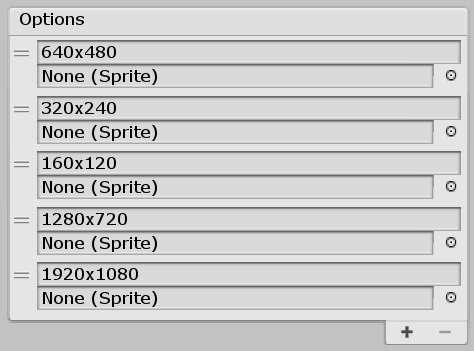
\includegraphics{/images/ai/dropdown.png}
\caption{}
\end{figure}

Then resize and position the dropdown on a place you'd like it to be on
the menu:

\begin{figure}
\centering
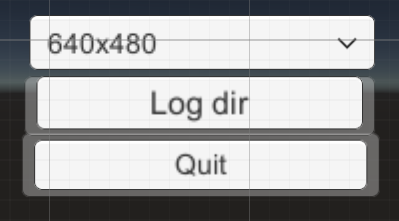
\includegraphics{/images/ai/dropdown2.png}
\caption{}
\end{figure}

Now go back to the \emph{Scripts} folder and add a new class called
\textbf{\emph{ResolutionSetter}}. This class will set the resolution
inside the \textbf{\emph{CameraSensor}} class based on the selected
option in the dropdown.

Here's the code for the \textbf{ResolutionSetter} class:

\begin{Shaded}
\begin{Highlighting}[]
\KeywordTok{using}\NormalTok{ System.}\FunctionTok{Collections}\NormalTok{;}
\KeywordTok{using}\NormalTok{ System.}\FunctionTok{Collections}\NormalTok{.}\FunctionTok{Generic}\NormalTok{;}
\KeywordTok{using}\NormalTok{ UnityEngine;}
\KeywordTok{using}\NormalTok{ UnityEngine.}\FunctionTok{UI}\NormalTok{;}

\KeywordTok{public} \KeywordTok{class}\NormalTok{ ResolutionSetter : MonoBehaviour}
\NormalTok{\{}
    \CommentTok{//Attach this script to a Dropdown GameObject}
\NormalTok{    Dropdown m\_Dropdown;}
    \CommentTok{//This is the string that stores the current selection m\_Text of the Dropdown}
    \DataTypeTok{string}\NormalTok{ m\_Message;}
    \CommentTok{//This Text outputs the current selection to the screen}
    \KeywordTok{public}\NormalTok{ Text m\_Text;}
    \CommentTok{//This is the index value of the Dropdown}
    \DataTypeTok{int}\NormalTok{ m\_DropdownValue;}
    \DataTypeTok{void} \FunctionTok{Start}\NormalTok{()}
\NormalTok{    \{}
        \CommentTok{//Fetch the Dropdown GameObject}
\NormalTok{        m\_Dropdown = GetComponent<Dropdown>();}
        \CommentTok{//Add listener for when the value of the Dropdown changes, to take action}
\NormalTok{        m\_Dropdown.}\FunctionTok{onValueChanged}\NormalTok{.}\FunctionTok{AddListener}\NormalTok{(}\KeywordTok{delegate}\NormalTok{ \{}
            \FunctionTok{DropdownValueChanged}\NormalTok{(m\_Dropdown);}
\NormalTok{        \});}
        \FunctionTok{setCameraSensorRes}\NormalTok{(m\_Dropdown.}\FunctionTok{options}\NormalTok{[m\_DropdownValue].}\FunctionTok{text}\NormalTok{);}
\NormalTok{    \}}

    \DataTypeTok{void} \FunctionTok{DropdownValueChanged}\NormalTok{(Dropdown change)}
\NormalTok{    \{}
       \FunctionTok{setCameraSensorRes}\NormalTok{(m\_Dropdown.}\FunctionTok{options}\NormalTok{[change.}\FunctionTok{value}\NormalTok{].}\FunctionTok{text}\NormalTok{);}
\NormalTok{    \}}

    \DataTypeTok{void} \FunctionTok{setCameraSensorRes}\NormalTok{(}\DataTypeTok{string}\NormalTok{ resolution)\{}
\NormalTok{        CameraSensor.}\FunctionTok{width}\NormalTok{ = System.}\FunctionTok{Convert}\NormalTok{.}\FunctionTok{ToInt32}\NormalTok{(resolution.}\FunctionTok{Split}\NormalTok{(}\CharTok{\textquotesingle{}x\textquotesingle{}}\NormalTok{)[}\DecValTok{0}\NormalTok{]);}
\NormalTok{        CameraSensor.}\FunctionTok{height}\NormalTok{ = System.}\FunctionTok{Convert}\NormalTok{.}\FunctionTok{ToInt32}\NormalTok{(resolution.}\FunctionTok{Split}\NormalTok{(}\CharTok{\textquotesingle{}x\textquotesingle{}}\NormalTok{)[}\DecValTok{1}\NormalTok{]);}
\NormalTok{    \}}
\NormalTok{\}}
\end{Highlighting}
\end{Shaded}

Now go back to the \emph{Scenes} folder and open the menu scene once
again. Select the dropdown element we created and in the inspector
panel, drag and drop the \textbf{\emph{ResolutionSetter}} script on it:

\begin{figure}
\centering
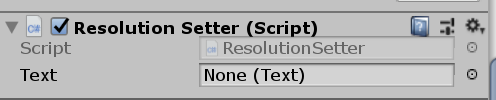
\includegraphics{/images/ai/dropdown3.png}
\caption{}
\end{figure}

And that's it. Now the output images will have the resolution that
you've set in the main menu using the dropdown.

\hypertarget{header-n43}{%
\subsubsection{Updating the default donkey-gym port}\label{header-n43}}

One thing we have to edit in donkey itself before we can use our modded
simulator:

\begin{itemize}
\item
  Go to your donkeycar project folder
\item
  Go to donkeycar/parts/ and open up \textbf{dgym.py}
\item
  Find the following line and change the port number from 9090 to 9091:

\begin{Shaded}
\begin{Highlighting}[]
\KeywordTok{def} \FunctionTok{\_\_init\_\_}\NormalTok{(}\VariableTok{self}\NormalTok{, sim\_path, port}\OperatorTok{=}\DecValTok{9091}\NormalTok{, headless}\OperatorTok{=}\DecValTok{0}\NormalTok{, env\_name}\OperatorTok{=}\StringTok{"whatever{-}env{-}name{-}here"}\NormalTok{, sync}\OperatorTok{=}\StringTok{"asynchronous"}\NormalTok{):}
\end{Highlighting}
\end{Shaded}
\end{itemize}

Now when you want to control your sim through the simulator
\emph{manage.py} script:

\begin{itemize}
\item
  Start it as you usually would, it should start the simulator
  automatically
\item
  Open the simulator and select the track you'd like the car to drive on
\item
  Click the \textbf{NN Control over Network} button
\item
  Open up localhost:8887 in a browser and you should be good to go!
\end{itemize}

\{\{\% notice tip \%\}\}

If you're compiling your model to a different directory than the default
one, or you've changed the project/executable name, be sure to update
the \textbf{myconfig.py} file, specifically the
\texttt{DONKEY\_SIM\_PATH} variable.

\{\{\% /notice \%\}\}

\hypertarget{header-n66}{%
\subsubsection{Building and using the modded
simulator}\label{header-n66}}

You can now go to File \textgreater{} Build Settings (or press CTRL +
SHIFT + B), select Build at the bottom of the screen and select the
folder where your simulator binary is. After building, you can use your
modded version the same way you used the default Donkey simulator
release.

Here's what a sample output image when the dropdown is set to 640x480:

\begin{figure}
\centering
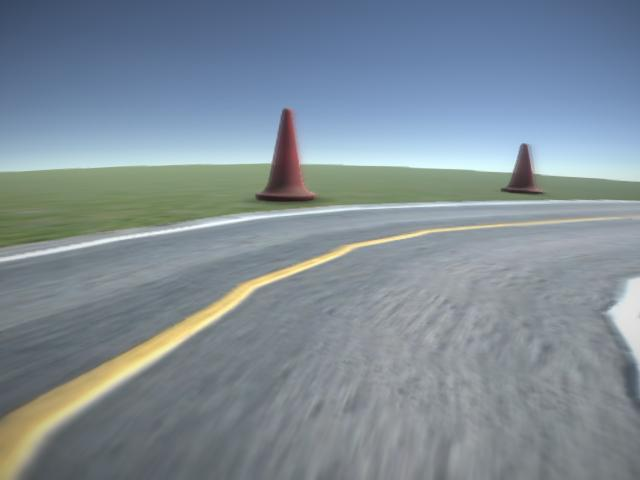
\includegraphics{/images/ai/480p.png}
\caption{}
\end{figure}

\end{document}
